\chapter{NDT graph-SLAM overview}
In this chapter we will present our solution to 2D version of the graph based \gls{SLAM} on the \gls{NDT} maps. This chapter starts with complete overview of the algorithm. In the next sections we explain how each part of the system is designed.
\section{System composition}
\label{sec:Sys_arch}

The standard input of many \gls{SLAM} algorithms is an odometry. In our case, we do not require any prior information about the robot movement. Our source of odometry is a fast incremental scan matching. The only mandatory input is a point cloud extracted from the robot's laser measurement. The scan matcher calculates relative transformation based on received point cloud and a  map from previous iterations of the incremental scan matcher. We will call this map a moving window. Details are in the section \ref{sec:window}.

The resulting transformation is used in the \gls{NDT} frame creation process. The \gls{NDT} frame is a small map which is created out of couple consecutive scans. A precise transformation is needed to merge these scans into a single frame. In our system, we use transformation from incremental scan matcher. The pose graph stores the \gls{NDT} frame inside the node. The \gls{NDT} frames integrate multiple scans to reduce the problem with the limited field of view. Each frame carries more information which gives a better outline of the world. More information about the world also helps to reduce a chance of ambiguous loop detections \ref{sec:Scan_reg} because larger frames have a higher chance to include some unique features. Additionally, we also want to utilize advantages of \gls{NDT-OM} occupancy update rule. It can detect dynamic objects with ray-tracing. The detection is done by merging multiple scans and re-observing the same cell multiple times.  More information about design choices behind \gls{NDT} frames is in the section \ref{sec:NDT_frame}.

 The next phase of the algorithm creates a node in the pose graph when the \gls{NDT} frame is created.  An odometry edge connects two consecutive nodes. The odometry received from scan matching process was used to create \gls{NDT} frames. Therefore, odometry edge has a transformation between origins of consecutive frames. In the next step, pose graph generates possible loop closure edges. The algorithm traverses a graph with Dijkstra projection and applies our radius based metric described in section \ref{sec:LoopClosureMetric}. 

The potential matches need to be registered and validated. It is the most difficult problem. We need an algorithm which can perform 10s of registration per second. At the same time, it needs to reject matches which are not from the same part of the environment.  Some errors caused by local and global ambiguities \ref{sec:Scan_reg} will not be avoided. We propose a solution to these problems by improving version of \gls{D2D}-\gls{NDT}. In this adaptation, we use a robust initial pose estimation from the correlative scan registration \ref{subsec:Corr} and fine alignment from \gls{D2D}-\gls{NDT} \ref{subsec:D2D_NDT}. The full description is in \ref{sec:Robust D2D-NDT}.

The loop closure edges need to be validated against possible outliers caused by ambiguities. We have decided to use a robust optimization engine with switchable constraints. We have made a decision based on the comparative study by \cite{RobustOpt}, where this method offered the best results. An important factor in optimization process is a number of nodes and edges in the graph. The computation time grows with increasing number of elements in the graph. We limit the number of nodes by using \gls{NDT} frames. Two consecutive frames can be farther away from each other because they represent a bigger part of the environment.

A Smaller number of nodes in the graph also mean less work to the \gls{NDT} mapper. In the case of successful loop closure, we need to regenerate map based on the new position of nodes in the graph. In this version of the algorithm, we just iterate over all frames and merge them to the new map based on the new origins. In the future \gls{NDT} frames allow to generate only a part of the map based on a request from a user. It could also be possible to load and save individual frames and save memory in the long run of the algorithm.

A combination of these parts together creates the graph-base \gls{SLAM} on the NDT maps.   

\begin{figure}
	\centering
	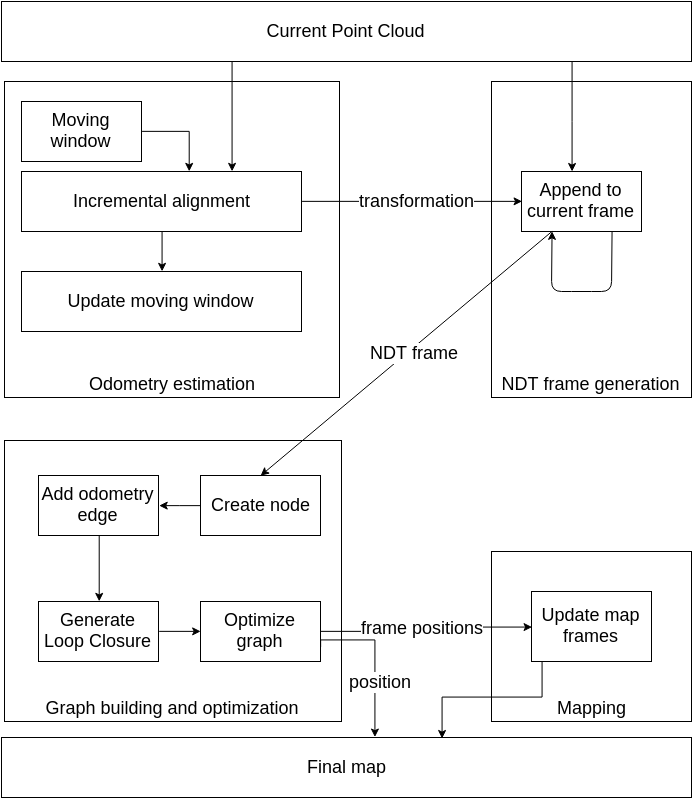
\includegraphics[width=100mm]{../img/algorithm_runtime.png}
	\caption{Diagram of graph based SLAM on NDT maps}
	\label{fig:algorithm}
\end{figure}
  
\newpage


\section{Moving window}
\label{sec:window}
A moving window is a special type of the \gls{NDT} grid. It uses all features of the \gls{NDT-OM} including the occupancy update and the dynamic object rejection. The main idea behind the moving window is to offer a small map which can be used by incremental scan matcher in order to efficiently align incoming scans against a longer history. In the standard incremental scan matching approach, we need to know the whole map. This map is then used to correct small errors when revisiting the same place again. A problem with this method arises when an alignment fails. In this case, the incorrectly aligned scan is merged into the map. It creates the same feature multiple times in the map. The next registration can use the wrong feature, and the error might never be corrected. The \gls{NDT-OM} can solve some of the degeneration by cleaning occupied cells which are on the way between robot position and the new measurement. In order for this mechanism to work, the next scan needs to converge to the original correct position. This is very unlikely with a corrupted map and the standard NDT technics for registrations, which can end up in the local optimum during the scan refinement step.

In our system, we do not need to know the whole map of environment because loops closures errors are fixed by pose graph optimization. We need incremental scan matcher to provide us a good local estimate of the robot movement. For this purpose, we only need to know the part of the environment overlapped with a current scan. It strongly depends on the type of a sensor and an environment. In our setup, robot operates in the indoor environment with laser sensor ranging up to 20m in long corridors. In this scenario window size of 20m should incorporate all information which can help in scan registration. If it is possible to select smaller window size based on the structure of the environment, the algorithm may save time and memory. 

The mowing window also needs to follow a movement of the robot to incorporate new measurements. It can be done in two ways. The first, we might rotate window based on exact changes of the robot global position. The algorithm must transform the whole window after each small movement of the robot. This approach tries to transform every single normal distribution inside grid in every step of the algorithm. Transformed cell's distribution may suddenly overlap multiple fields. We would need to develop a mechanism how to split original distributions into the multiple cells. A better way is to keep windows orientation fixed and only translate the window based on the robot's movement. It prevents a rotation of distributions in the cells but still, suffers from the same splitting problem. The final solution is to move the window only in multiples of the cell size. It does not affect parameters of normal distribution inside of original grid when the window moves multiple fields in any direction. After the movement, some cells may get out of the scope of the current window. These cells are destroyed which help to reduce accumulated error in the window.

To minimize any alignment issues we have decided to perform fast scan matching. We achieve it by processing as many laser scans as possible. The high-frequency scan matching does not need initial guess because a valid result is reasonably close to the initial position of the source and the target measurements. The registration algorithm which is capable of this performance needs to work in order of milliseconds. Two algorithms developed for fine registration on top of the \gls{NDT} grid are the \gls{P2D}-\gls{NDT} and the \gls{D2D}-\gls{NDT}. We use the standard \gls{D2D} algorithm because it offers ten times better run time than \gls{P2D}. A comparative study by \cite{NDTcomparative} shows that even though \gls{P2D} is usually more precise, it needs significantly more computation time. Skipping multiple measurements from the sensor may cause that we will not be able to estimate robustly transformation and the whole process can converge to a local minimum. 

\begin{algorithm}
\label{alg:move_window}
    \caption{Moving window processing loop}
\begin{algorithmic}[1]
\Require point cloud $X$, move window's \gls{NDT} grid $M$, transformation $T_{o}$ to the origin of moving window, transformation $T_{r}$ unused from move in last call of function, transformation $P$  last known absolute pose of moving window.  
 \Function{calculateTransform}{$X$}
	 \State $X_{o} \gets$ transformPointCloud($X$,$T_{o} * T_{r}$)
	 \State $N_{o} \gets$ createNDTGrid($X_{o}$)
	 \State $T_{ox} \gets$ alignD2D($N_{o}$,$M$)
	 \State $M$.mergeIn($X_{o}$,$T_{ox}$)
	 \Comment applies transformation on point cloud and merge it into moving window
	 \State $T_{diff} \gets P^{-1} * (T_{o} * T_{ox})$
	 \State $P \gets T_{o} * T_{ox}$
	 \Comment update of absolute pose of window for next call 
	 \State $T_{r} \gets M$.moveWindow($T_{ox}$)
	 \State \Return $T_{diff}$
 \EndFunction
\end{algorithmic}
\end{algorithm}
\todo{add visualization of running window}

\newpage

\section{NDT frame creation}
\label{sec:NDT_frame}
The \gls{NDT} frame is created by merging multiple point clouds based on transformation received from odometry estimation. The important question is how many scans should we combine? This algorithm uses consecutive addition of transformation as in equation \ref{eq:concat_trans}. Afterward, it calculates a total displacement done by a robot. If it is more than a threshold we close down the old \gls{NDT} frame and start to add scans into the new empty frame. The new frame is assigned its coordinate system based on current robot position. Every new scan is transformed into the coordinate system of currently opened frame and merged in. The closed frame is sent to the pose graph generation where it is transformed into the node.

A Selection of good displacement parameter is important for a run of the algorithm. A small value will create many nodes in the pose graph. Every node will reflect an only small portion of the environment. This will make loop closure computationally expensive by a need to evaluate too many possible loop closure nodes. At the same time, loop closing algorithm will work with only limited information. This may cause a bigger number of local and global ambiguities in registration. A large value of displacement will generate fewer nodes with more information in each node. This is less computationally dependent. On the other hand, it creates an ambiguous environment inside of the \gls{NDT} frame. The loop closure registration may not correctly deduce which part of the same environment in the frame is correct for registration. The registration algorithm is forced to identify this situation and solve it. At the same, it wastes an optimizer's potential in ambiguity rejection based on topological information of the whole environment. 

\section{Loop closure detection}
\label{sec:LoopClosureMetric}
A loop closure detection is done on top of the pose graph. The loop detector can use current positions of the graph nodes and relative transformations stored in the odometry and loop closure edges. With this information, we need to find all nodes which can with current node create a loop closure edge. The process starts by Dijkstra projection mentioned in the section \ref{subsec:loop_closure_creation} from the current node. A part of the projection is also a calculation of the relative displacement along the edge. The sum of displacements is used as a parameter for rejection of nodes which are too close to our current position. These nodes are certainly overlapping with our start node and therefore it is not necessary to check them again. All the nodes passing the previous test are used in one of two rejection models. 

The first model tests all nodes against selected radius. The second mechanism is using cumulative transformation and covariance calculated by Dijkstra projection. In validating if two nodes overlap we use same metric as presented by \cite{Olson2009Loop}.
\begin{equation}
\varDelta c = (c_{b} - c_{a})
\end{equation}
\begin{equation}
s  = \max(0,\lVert \varDelta c\rVert - r_{a} - r_{b})\frac{\varDelta c}{\lVert \varDelta c\rVert}
\end{equation}
\begin{equation}
mahl = s^{T}P_{a,b}^{-1}s
\end{equation}
where $c_{a}$ and $c_{b}$ are the centroids of start and currently compared \gls{NDT} grids; $r_{a}$ and $r_{b}$ are radii of the respective \gls{NDT} grids and $P_{a,b}^{-1}$ is an inverse of the accumulated covariance.
 
The selected nodes are registered by robust \gls{D2D}. Those matches with high score are inserted into the graph. The edges added by this mechanism may still include some errors or ambiguities. Rejection of these edges is done in the optimizer.


\section{Robust D2D-NDT registration}
\label{sec:Robust D2D-NDT}
Construction of a robust \gls{D2D} registration needs to be fast and precise. Also, it needs to have a mechanism how to reject invalid association. It can use only information present in \gls{NDT} grids because a loop closure mechanism is working only with this data. We knew that the \gls{D2D} offers quick and reliable registration on the \gls{NDT} grids with a good initial guess. The correlative scan matching algorithm  \ref{subsec:Corr} can provide registration without a knowledge of the initial guess. Unfortunately, in the standard version, it is not possible to operate with \gls{NDT} grids. The performance of this algorithm is also slower than \gls{D2D}. To solve these problems we have developed modified version of the correlative algorithm which can work on top of \gls{NDT} grids.

\subsection{Adaptation of correlative registration}
We have started with the base algorithm described in the section \ref{subsec:Corr}. It is sufficient for our needs when this algorithm provides only a rough initial guess. For this reason, we use only one layer architecture. Our single grid has double cell size in comparison with the original size of the \gls{NDT} grid. It offers faster execution time. In the first part of the algorithm, we need to go over large search space because we cannot expect any prior information from the graph. Larger grid size limits the number of translation because we always try translations in multiple of the cell size as mentioned in the \ref{subsec:Corr}. 

Secondly, we need to transfer original \gls{NDT} grid into a reasonable point cloud. In our implementation, we have decided to recreate point cloud out of grid by taking a mean from every cell with distribution. A collection of these means makes our mean cloud. In addition, we use information about how many points were used to create a normal distribution. This information is used in our algorithm as a weight for every mean value. Original algorithm uses two point clouds. 

First is called target cloud and is used for the creation of look up table. This table is created by projecting all points to individual cells. When is a cell occupied by at least one point it is marked with value 1. In our scenario, we use a cloud of means from the target grid to construct a look-up table. Use of means is more robust to outliers than original look-up table from a point cloud. The original implementation marked every cell occupied regardless on the number of points mapped into it. Our grids need at least 4 points to create a normal distribution. This limits an influence of the single point spread in a space and also emphasizing dominant structures in the environment. Target grid conversion to mean cloud does not loose any information in comparison to the original cloud. This is because the look-up table and the target grid are aligned. On top of that double step size of the look-up table makes four cells from the target \gls{NDT} contribute to a single look-up cell.
  
The second source cloud is used for scoring in the look-up table. Every point of a point-cloud contributes to total score based on the value from the look up cell it belongs to. In our case, the single point represents information about the mean center of multiple points. In order to keep all information, algorithm maps mean into the correct cell in the look-up table. By doing this, the mean only contributes once. Fortunately, a score generated by mean can be scaled with the use of weight associated with the mean. This makes a weighted mean point contribute the same amount to the system as standard points from point cloud. The score function is defined as:
\begin{equation}
score(T,C) = \frac{1}{d}\sum_{p \in C}^{} v(T,p) w(p) 
\end{equation}

where $T$ is transformation which should be applied to point $p$ of cloud $C$. A function $v(T,p)$ applies transformation $T$ to point $p$ maps it to look up table and return score value for single point. A function $w(p)$ return weight of current mean point. Scaling factor $d$ is defined as
\begin{equation}
d = m\sum_{p \in C_{t}}^{}w(p)
\end{equation} 
where $m$ is the maximal value one point can receive from look up table after application of smoothing kernel in equation \ref{eq:smooth_kernel}; $C_{t}$ represents target point cloud. 

The last problem with conversion of source cloud to mean cloud is to handle discretization errors. These errors happen when we need to transform \gls{NDT} grid. In this situation, one original \gls{PDF} may overlap multiple cells. The original point cloud would contribute into multiple cells. Our mean formulation would contribute only to one cell based on mean location. To minimize this effect, we map every mean value into the target look-up table which has double cell size in comparison with source \gls{NDT}. This process is similar to multi-layer discretization removal in multi-layer \gls{NDT} registration \cite{ulas20113d}. The Target look up table also include a smoothing kernel, which assigns some value to cells surrounding occupied cell in the table. This also makes mean which could potentially slip out of occupied cell's boundaries contribute to the total score.

By executing these approximations, we were able to create a version of the correlative registration on top of \gls{NDT} grids. Coarser resolution improved performance and allowed us to search larger search space. Approximation of the input cloud into means reduce the number of a point we need to test in every iteration of the algorithm loop. This effectively lowered number of calls to the look-up table, which speeds up the whole process. In addition, mean cloud removes outliers from the points spread in space.


\subsection{Algorithm overview}
With the coarse initial guess estimate, we can construct the algorithm. The first step is to run correlative estimation algorithm on a pair of grids. The result is the best initial guess it could find in the selected search space. The correlative estimator uses a coarse look-up table which means that grid still needs to be transformed up to two \gls{NDT} cell. The next step is to run the \gls{D2D} algorithm. The multi-layer definition of the \gls{D2D} can converge to the right solution if there is one. The problem arises if two matched grids are from different locations and do not share same environment features, e.g., lines, corners. In this case, correlation registration finds the best possible solution, which means that it rotates grid in a way that maximalizes a score. The \gls{D2D} than try to find the best alignment and usually falls to the first local minimum it can find. To solve these situations we propose solution validation process. Example of bad alignment is in figure \ref{fig:bad_align}. 



\subsection{Solution validation}
Robust alignment offers us the best transformation between the source and the target \gls{NDT} grid. This alignment can fail and not provide a successful registration at all. We need to validate if this registration succeeded or failed. In this algorithm, we again use correlative scan matcher. In this case, we use a cell size of the target look-up table matching the cell size of the \gls{NDT} target grid. We map every point from mean source cloud into a look-up table and receive a total score based on contributions of each weighted mean point. In this case, discretization is helping us to provide better results. Some means may stay out of the target grid this means that registration was less successful which result in a lower score. This method can reject scans based on their overlap. It is not able to distinguish the wrong alignment in case that two scans look similar but originate in two different parts of the environment. This ambiguity is resolved in the graph.

\begin{algorithm}
\label{alg:robust_d2d}
    \caption{Robust \gls{D2D} registration algorithm}
\begin{algorithmic}[1]
\Require source \gls{NDT} grid $G_{s}$ and target \gls{NDT} grid $G_{t}$. Resolution of \gls{NDT} grids $r$. Validation threshold $v$
 \Function{align}{$G_{s}$, $G_{t}$, $r$}
 \State transformation T is identity
 \State ($T$,$score$) $\gets$ correlativeEstimater($G_{s}$, $G_{t}$,$T$, $2*r$)
 \State $T \gets$ alignD2D($G_{s}$, $G_{t}$,$T$)
 \State ($T$,$score$) $\gets$ correlativeEstimater($G_{s}$, $G_{t}$,$T$, $r$)
 \If{$score \geq v$}
	 \State \Return ($T$,$true$) 
 \Else
	 \State \Return ($T$,$false$)
 \EndIf
 \State \Return T 
 \EndFunction
\end{algorithmic}
\end{algorithm}

\begin{figure}
	\centering
	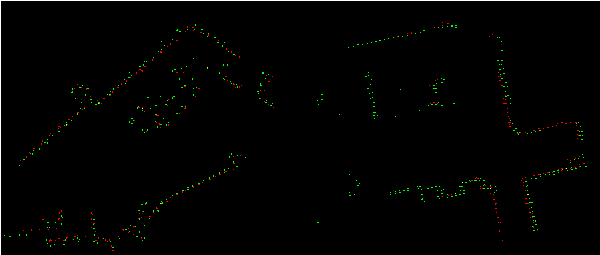
\includegraphics[width=150mm]{../img/good_align.png}
	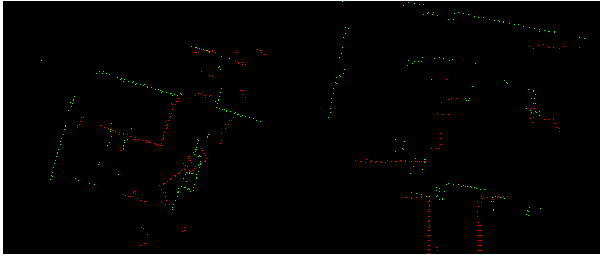
\includegraphics[width=150mm]{../img/bad_align.png}
	\caption{Images with alignment. Red dost represent target scan and green dots source scan. The first row shows valid alignment marked with high score. Second row shows two alignments which were rejected by validation.}
	\label{fig:bad_align}
\end{figure}
\newpage
